\section{Bayesian neural network regression}\label{BNN} 

Neural networks have become increasingly popular in recent years, due to their ability to
approximate any function arbitrary well (showed via the universal approximation theorem) and with
the amount of data in the world today, neural networks are very powerful regression models for
finding complex patterns. Bayesian neural networks are essentially neural networks, but instead of
point estimates, each weight is assigned a distribution, which provides a probabilistic regression
model (see Figure \ref{BNN_illustration2}). Prior to any observed data, the weights are assigned a
distribution (typically a standard Gaussian). After observing data a joint (posterior) distribution
of the weights are inferred, such that the regression model is fitting the data and provides good
uncertainty estimation (note that the weights might be complicated and correlated). In Figure
\ref{BNN_prior_posterior} we see how the regression model can do predictions even when no data is
observed, i.e. prior samples (left), when observing data the posterior combines the likelihood and
the prior and we get the predictive posterior distribution (right). 
\begin{figure}[H]
    \subfloat{{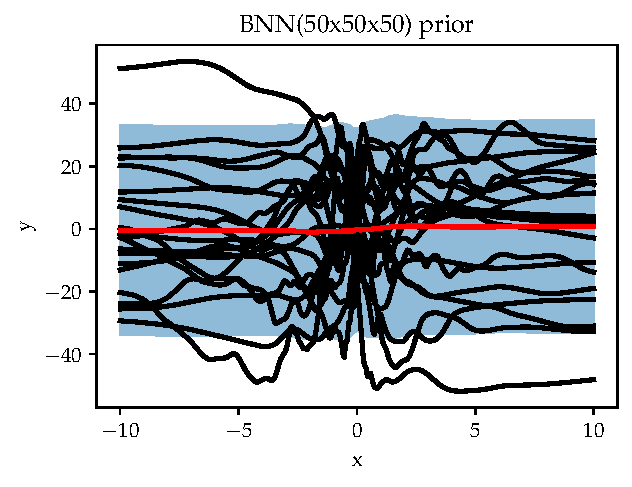
\includegraphics[width=0.45\textwidth]{Pictures/BNN_prior.pdf} }}%
    \qquad
    \subfloat{{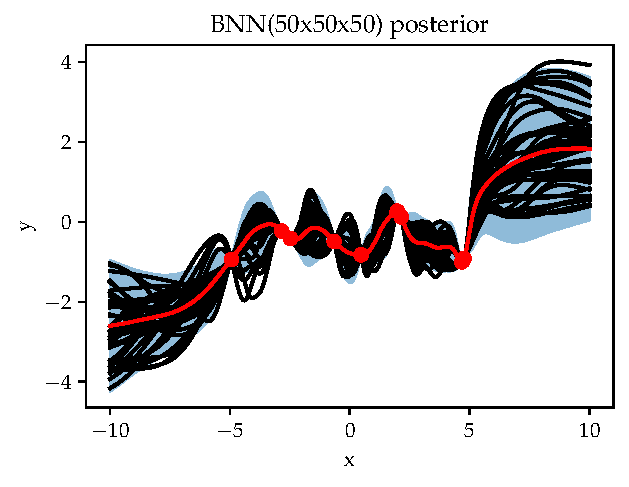
\includegraphics[width=0.45\textwidth]{Pictures/BNN_posterior.pdf} }}%
    \caption{Left: 20 black predictive \textit{prior} samples from a 3 layers BNN with 50 $\tanh$ nodes, with standard Gaussian prior distributions. 
     Right: 20 predictive \textit{posterior} samples. The blue areas are $\pm$ 2 predictive standard
     deviations from the red predictive mean.}%
    \label{BNN_prior_posterior}%
\end{figure}

\begin{figure}
    \centering
    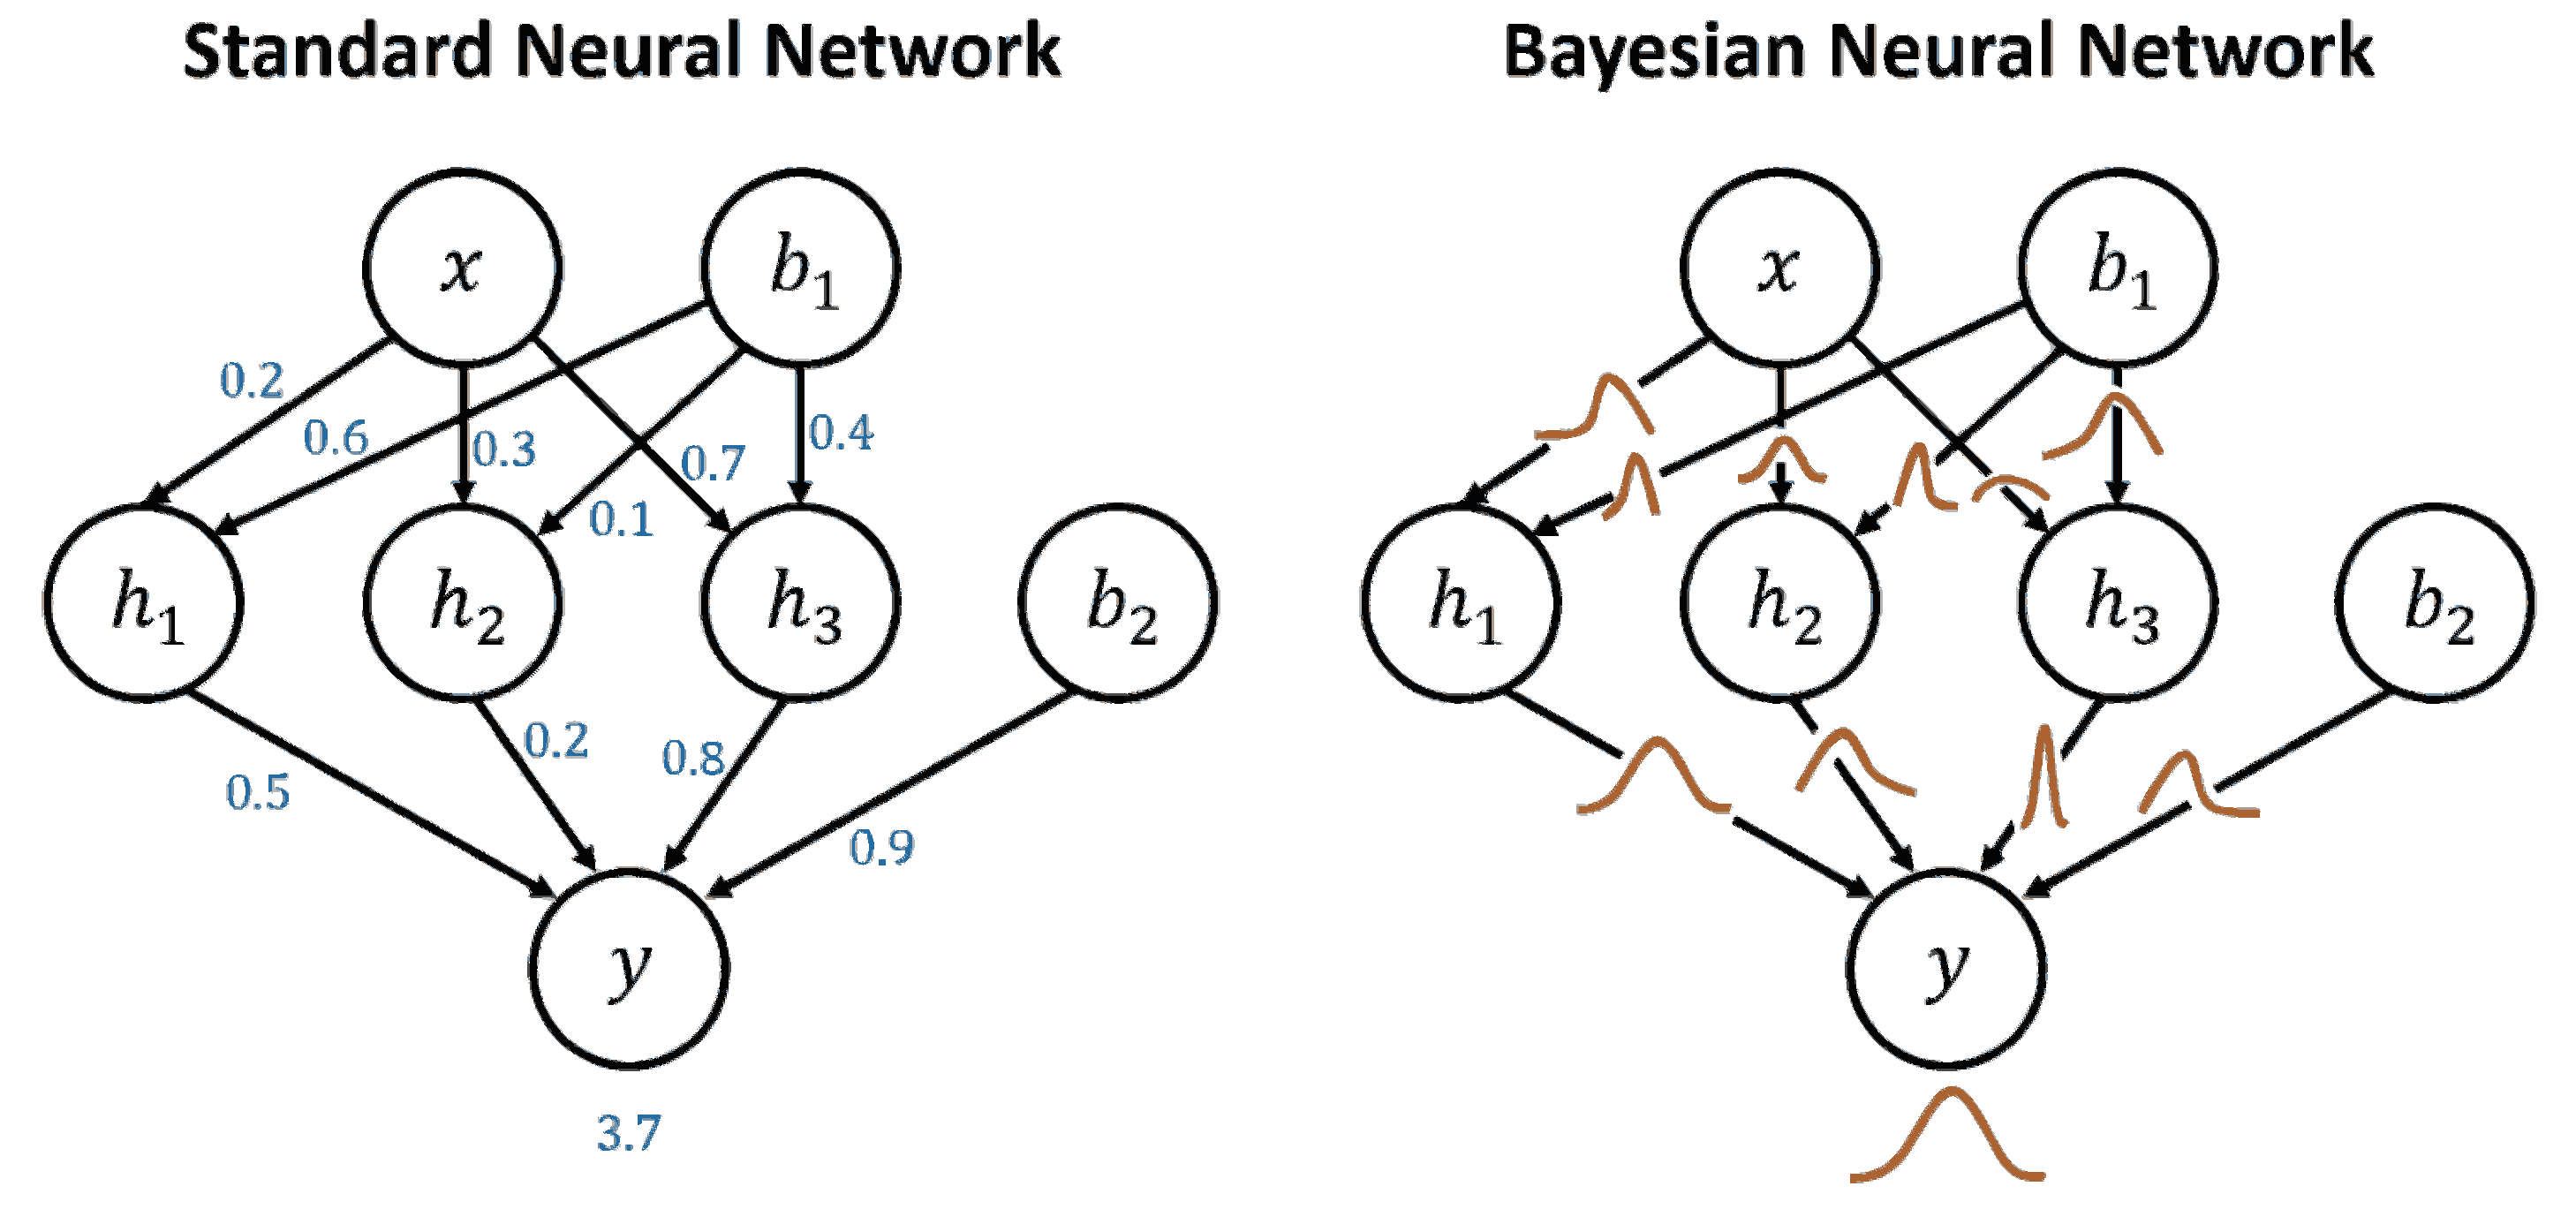
\includegraphics[width=\textwidth]{Pictures/BNN_illustration.pdf}
    \caption{Graphical representation of a Bayesian neural network compared to a neural network. The
    weights are assigned a probability density. Note that we often prior assume no correlation and
    a standard normal distribution, but the posterior (after observing data) might contain
    correlations between the weights.}
    \label{BNN_illustration2}
\end{figure}

The likelihood of a Bayesian Neural network is typically defined as a normal distribution with mean
equal the neural network output and a observation variance $\sigma^2$ (both are random variables) which in the
thesis is assumed constant throughout the domain.  
$$p_{\text{\tiny BNN}}(y|x, \theta) = \mathcal{N}(y|f_{\textbf{w}}(x),\sigma^2)$$


The prior distribution of the weights (including the biases) are typically assumed uncorrelated
standard normal distributed and the observation variance $\sigma^2$ can be assigned a lognormal or
half-Cauchy, with support on the positive real domain. We can write the priors of the BNN model as
\begin{align*}
    p(\theta = (w, \sigma)) &= \mathcal{N}(w;\textbf{0},I) \log\mathcal{N}(\sigma;\dots)
\end{align*}
Now we can define the posterior distribution, i.e. the probability of the unknown quantaties given
the observations. We define it using Bayes rule, 
\begin{align*}
    p(\theta|x,y) &= \frac{p(\theta,y|x)}{p(y|x)}\\
    &=\frac{p_{\text{\tiny BNN}}(y|x, \theta)p(\theta|x)}{p(y|x)}.
\end{align*}
Note that the prior distribution $p(\theta|x)$ just like the likelihood can depend on $x$ - we could
for example extend $\sigma$ to depend on the location of the sample $x$ and define it as
$\sigma(x)$. Note that the posterior distribution of the weights and $\sigma^2$ is
complex and correlated due to the multiplication of the compllicated likelihood and the prior. 
Therefore, exact inference of BNNs is intractable and we approximate the predicitve posterior distribution 
with Monte Carlo samples from posterior, 
\begin{align*}
    p(y_*|x_*,\mathcal{D}) &= \int p_{\text{\tiny BNN}}(y_*|x_*, \theta)p(\theta|\mathcal{D})d\theta\\
    &\approx \frac{1}{K} \sum_{k=1}^K p_{\text{\tiny BNN}}(y_*|x_*, \theta^{(k)})
\end{align*}
where the integral is intractable. As indicated in the second line, we can approximated the integral
with Monte Carlo sampling: $\theta^{(k)}$ are independent and identical (iid) samples from the
posterior distribution, $\theta^{(k)} \sim p(\theta|\mathcal{D})$. 
\begin{testexample2}[Monte Carlo approximation]
    Assuming we have a number of iid samples, $\theta^{(1)}, \dots, \theta^{(K)}$ drawn from the
    distribution $p(x)$, then the following appriximation $$E[f(x)] \approx \frac{1}{K} \sum_{k=1}^K
    f(x^{(k)}) =: \Theta_{K}(f)$$ holds according to the law of large numbers. In fact,  $$E[f(x)] =
    \lim_{K \rightarrow \infty} \Theta_{K}(f)$$ and the central limit theorem ensures that the
    variance of the unbiased estimator of the expectation decreases with number of samples, $K$, i.e.
    $$p(\hat \Theta)  \approx  \mathcal{N}(\hat \Theta |\mu_f,
    \frac{\sigma_f^2}{K}),$$ where $\mu_f := E[f(x)] $ and $\sigma_f^2 =
    Var(f(x))$. \cite[708]{ML_Bayesian_Pespective}
\end{testexample2}
We aim to get (approximately) iid samples from the posterior distribution using MCMC. However,
is it rarely the case that MCMC achieve iid samples. Therefore, more samples are necessary to acieve the same results. The
closer to iid the samples are the less samples are needed \cite[12]{MCMC}.

\subsection*{Posterior samples}
For BNN the joint distribution $p(\mathcal{D},\theta)$ is available, but calulating the posterior
distribution requires the marginalized likehood, $p(\mathcal{D}) = \int_{\theta}
p(\mathcal{D},\theta)$. This integral is often intractable since the space of $\theta$ typically is
abnomous - so not even nummerical approximations of the intergral is tractable. From Bayes rule, we
have the equality, 
$$p(\theta|\mathcal{D}) = \frac{p(\mathcal{D},\theta)}{p(\mathcal{D})} \propto
p(\mathcal{D},\theta),$$ where the propotional sign is true, since $p(\theta|\mathcal{D})$ is a
function of $\theta$. Knowing the joint distribution, $p(\mathcal{D},\theta)$, allow for using Markov
chain Monte Carlo (MCMC) to obtain samples from the posterior distribution.  

\begin{testexample2}[Markov chain Monte Carlo (MCMC)]
    We can use MCMC for sampling from a probability density $p(x)$, with only the knowledge of a 
    proportional/unnormalised density $\hat p(x) \geq 0$ i.e
    $$\hat p(x) = c\cdot p(x) \propto p(x), \hspace{1cm} c = \int \hat p(x) dx,$$ where $\int \hat
    p(x) dx$ may be intractable. The MCMC procedure constructs an \textbf{ergodic} Markov
    chain/process, such that its \textbf{stationary} distribution is exactly $p(x)$, but only with
    the knowledge of $\hat p(x)$. Here is a short explaination of the ergodicity and stationary (from
    \cite[540]{bishop}):
    \begin{itemize}[noitemsep]
        \item \textbf{Ergodicity}: A Markov chain which spans/visits all the space. 
        \item \textbf{Stationarity}: A Markov chain is stationary if each step in the chain leaves
        the distribution unchanged, implying that samples from the distribution remain samples from
        the same distribution after each step.
        % A Markov process has reached stationary distribution if
        %                     we stay there at the next sample. 
        \item \textbf{Detailed balance relation}: A sufficient condition to check if a Markov chain
        is stationary is by the detailed ballance equation: $$p(x)p(x\rightarrow y) =
        p(y)p(y\rightarrow x).$$ Note we introduce the notation $p(x\rightarrow y)$ for the
        transition probablity from x to y, this can also be interpreted as a conditional
        distribution of state $y$ given state $x$  
    \end{itemize}
\end{testexample2}
So since the known joint distribution is proportional to the posterior distribution, we can use MCMC
to get samples from the posterior distribution, even when it is intractable. To better introduce
what MCMC is, we here present a simple MCMC procedure, the Metropolis-Hasting algorithm (HM), and
give proof of why its produced Markov chain stays in its stationary distribution.

\begin{testexample}[MCMC example: Metropolis-Hasting (MH)]
     At iteration $n$ we already have a sample $x_n$,
    \begin{enumerate}
        \item Propose $\hat x$ from a proposal density $q(\cdot|x_n)$
        \item Compute acceptance probability $$\alpha(x_n,\hat x) = \min \left(1, \frac{p(\hat
        x)}{p(x_n)} \frac{q(x_n| \hat x)}{q(\hat x|x_n)}\right)$$
        \item Set the next sample $$x_{n+1} = \begin{cases}
            \hat x &\text{with probability } \alpha(x_n, \hat x)\\
             x_n &\text{with probability } 1-\alpha(x_n, \hat x)
        \end{cases}$$
    \end{enumerate}
    note that $\alpha(x_n,\hat x)$ uses $p(x)$ in the fraction $\frac{p(\hat x)}{p(x_n)} =
    \frac{p(\hat x)\cdot c}{p(x_n)\cdot c} = \frac{\hat p(\hat x)}{\hat p(x_n)}$, so we only need $\hat
    p(x)$.  
    
    \textbf{Proof:} Assuming discrete states, the transition probability between the states are given as, 
    $$p(x\rightarrow y) = \begin{cases}
        q(y|x)\alpha(x,y) & \text{if } x\neq y\\
        q(x|x) + \sum_{z\neq x} q(z|x)(1-\alpha(x,z)) & \text{if } x=y
    \end{cases}$$
    Now, let us look at the detailed balance relation. Assume $x\neq y$, 
    \begin{align*}
        p(x)p(x\rightarrow y) &= p(x)q(y|x)\alpha(x,y)\\
        &=p(x)q(x,y) \min \left(1, \frac{p(\hat x)}{p(x_n)} \frac{q(\hat x, x_n)}{q(x_n,\hat x)}\right)\\
        &= \min(p(x)q(x,y), p(y)q(y,x))
    \end{align*}
    Observing that the right hand side yields symmetric result in $x$ and $y$, therefore we obtain, 
    $$p(x)p(x\rightarrow y) = p(y)p(y\rightarrow x)$$
    and summing over $x$ on both sides yields,
    \begin{align}
        \sum_x p(x)p(x\rightarrow y) &= p(y) \sum_x p(y\rightarrow x)\\
        \implies \hspace{0.5cm} p(y) &= \sum_x p(x)p(x\rightarrow y).
    \end{align}
     The detailed balance is trivially obtained for $x = y$, all in all, this reveals that $p(x)$ is in fact
     invariant for the chain $\{x_1, \dots , x_n\}$ and thereby that MH is a MCMC algorithm. 
\end{testexample}
% Markov assumption -> history doesn't matter
% Monte Carlo -> Random simulation
% best methods, use gradients. 
% Simulared skate board in a state park. Physic simulation. 
% Often the simulation moves back and fouth and end up in the 
% same point - this is called a U-turn. 
% find global curvature from just knowing the local curvature. 
% Simulation is moving more in the area with high prob. mass. 
% Gradients: Automated differentiation. 
% We want to evaluate integrals of the fom $$E[f(x)] = \int f(x)p(x)dx$$ where $x \in \mathbb{R}^n$ is a
% random vector under the distribution $p(x)$. we are interested in problems where the form of $f(x)$ or $p(x)$
% makes the integral intractalbe. 
% \begin{testexample}[Bayesian neural network]
%     Choosing $f := \mathcal{N}(y;NN_w(x), \sigma)$ and looking at $\theta := (w,\sigma)$ as the random quantaty
%     under the posterior distribution $p(\theta|\mathcal{D})$ we indeed have case of a intractalbe expectation
% \end{testexample}
% Transition density kernel (transtion matrix for finite discrete spaces) $p(x^{(k)}|x^{(k-1)})$
% c) the convergence rate is independent on the
% dimensionality, l. The latter property is in contrast to methods based on the deterministic numerical
% integration, which, in general, have a rate of convergence that slows down as the dimensionality
% increases.
HM with its random walk transition is very simple and it comes with some serious disadvantages: Slow
convergence speed, it might stay in the same region for a long time and produce highly correlated
samples(i.e. not the iid samples we need for the Monte Carlo approximation to be correct) \cite[]{ML_Bayesian_Pespective}.
The gold standard in MCMC, Hamiltonian Monte Carlo (HMC), replaces HMs random walk with
gradient-guided movements and interpret the probability landscape as a physical system.
 
\begin{testexample}[Hamiltonian Monte Carlo (HMC)]
HMC exploits arguments from classical mechanics around the Hamiltonian equations.
This method leads to more efficient sampling as the Hamiltonian interpretation allows the system to
consider regions with high probability more - this is obtained using a gradient of the probability
landscape, $\frac{-\partial E(x)}{\partial x} $.
 
We introduce the potential energy $E(x)$ by defining the joint probability as, 
$$p(x) = \frac{1}{Z_E}\exp(-E(x))$$ Now, a latent vector $q$ is introduced in order to represent the
momentum of the system, which gives us the kinetic energy of the system. 
$$K(q) = \frac{1}{2}\sum_{i=1}^l q_i^2$$ Combining the kinetic and potential energy yields, the the
Hamilton function and its corresponing distribution
$$H(x,q)= E(x)+K(q)$$
and 
\begin{align}
    p(x,q) &= \frac{1}{Z_H} \exp(-H(x,q))\\
    &= \frac{1}{Z_E} \exp(-E(x))\frac{1}{Z_K} \exp(-K(x))\\
    &= p(x)p(q)
\end{align}

The desired distribution $p(x)$ is found as the marginal of $p(x,q)$.
The sampling procedure is as follows, 
\begin{enumerate}[noitemsep]
    \item At the $(x_n,q_n)$ sample momentum $q_n$ by gibbs sampling
    \item Simulate the Hamiltonian dynamics with Leap-frog integration (i.e. walking the contour lines of $p(x,q)$).
    New position is $(x_{n+1}, q_{n+1})$
    \item Accept new position with MH acceptance probability $\min(1,\frac{p(x_{n+1}, q_{n+1})}{p(x_{n}, q_{n})} )$
\end{enumerate}
We refer to \cite{neal} for proof that HMC is indeed a MCMC. 
\end{testexample}

\subsection{MCMC used in thesis}
While being a popular sampling method for BNN inference, Hamiltonian Monte Carlo is very
sensitive to the two parameters used in the leapfrog integration (physical simulation): the step
size and the number of steps. These parameters are typically tuned by conducting a
number of initial experiments, i.e. data set samples, which is not appropriate in a BO setting with
an expensive objective function. The NUTS sampling method (No-U-Turn-Sampler) \cite{NUTS}
is an adaptive version of HMC, which terminates the leapfrog integration when the simulation reaches
the starting point. Thereby we avoid manually tuning of the number of steps.

The paper \cite{BOHAMIANN} introduces a Bayesian optimization framework called Bayesian Optimization
with Hamiltonian Monte Carlo Artificial Neural Networks (BOHAMIANN), which demonstrates state of the art
performance on a wide range of optimization task. It is stochastic gradient HMC where the hyperparameters
are tunes adaptively doing the burn-in phase. It is implemented using 


% JEG OVERSÅ dette: 
%  Wrapper around pybnn Bohamiann implementation. It automatically adjusts the length by the MCMC chain,
% by performing 100 times more burnin steps than we have data points and sampling ~100 networks weights.

% We now show Bayesian optimization experiments for BOHAMIANN. Unless noted otherwise,
% we used a three layer neural network with 50 tanh units for all experiments. For the priors we
% let p(θµ) = N (0, σ2
% µ
% ) be normally distributed and placed a Gamma hyperprior on σ
% 2
% µ
% , which is
% periodically updated via Gibbs sampling. For p(θ
% 2
% σ
% ) we chose a log-normal prior. To approximate EI
% we used 50 samples acquired via SGHMC sampling.


% We found the
% friction term and the step-size to be highly model and data-set dependent3
% , which is unacceptable for
% BO, where robust estimates are required across many different functions F with as few parameter
% choices as possible.

% Historically, Hamiltonian Monte Carlo (HMC)
% [157] has been the most popular sampling method used in BNNs. However,
% its performance is very sensitive to a proper initialization of its two user-
% specified parameters, namely step size and number of steps, which are
% normally set by carrying out a number of initial experiments. This makes
% HMC inappropriate for the Expensive Optimization application, where new
% observations are incrementally added and the surrogate model undergoes
% change in each iteration. Fortunately, the No-U-Turn-Sampler (NUTS) [86],
% an adaptive version of HMC, resolves this limitation by eliminating the
% need for setting the number of steps in advance.
\subsection{Design and properties of Bayesian neural network}
The architecture of a BNN is a large topic to discuss. There are certain tradeoffs to be taken into
consideration: How expressive should the network be (i.e. how deep and how many nodes per layer)
versus how much time do we have for the sampler to converge to the true posterior distribution? A
challenging part of MCMC is that it is difficult to know when the samples are true samples from the
posterior. A consideration when training deterministic neural networks are overfitting however this
is not a big consideration when fitting Bayesian neural networks; Choosing a prior around 0 will
regulate the parameters, and thereby postpone overfitting. 

This thesis is inspired by the PhD thesis \cite{PhDthesis}, which uses an architecture of a 2 layers
with 50 sigmoid nodes in each layer, and the BOHAMIANN paper \cite{BOHAMIANN}, default uses an architecture
of 3 layers with 50 tanh-nodes in each layer. As we want to make sure always to do the 
inference correctly, we want to be able to take a proper amount of samples, while also
having an explicit model. Figure \eqref{n_unit_BNN} shows prior samples of BNN with a different
number of tanh-nodes on each of the 3 layers, this provides an intuition that choosing a larger
BNN leads to a more expressive regression model. When doing Bayesian optimization the model as a small
amount of training data, i.e. complicated patterns in data is not possible to discover, and hence 
highly expressive models are not important. 

\begin{figure}[H]
    \centering
    \begin{minipage}[b]{0.24\textwidth}
     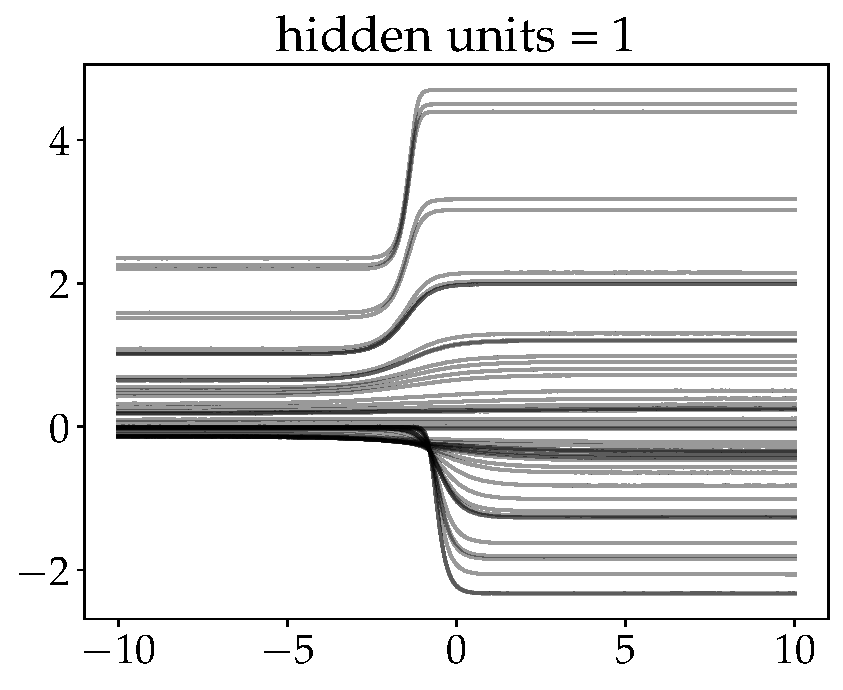
\includegraphics[width=\textwidth]{Pictures/bayesian_nn_prior_samples_hidden_units_0.pdf}
    \end{minipage}
    \hfill
    \begin{minipage}[b]{0.24\textwidth}
     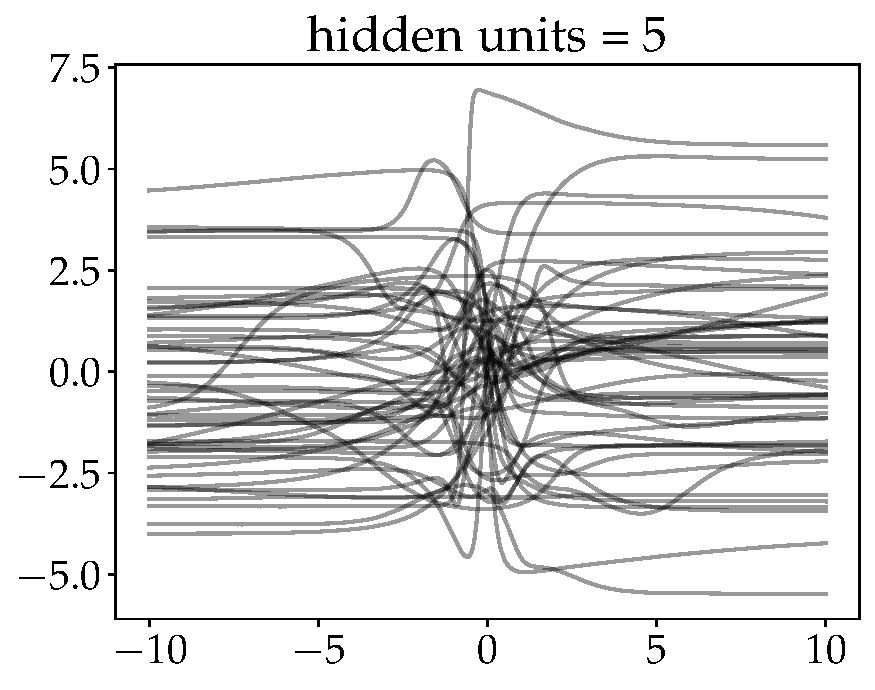
\includegraphics[width=\textwidth]{Pictures/bayesian_nn_prior_samples_hidden_units_1.pdf}
    \end{minipage}
    \hfill
    \begin{minipage}[b]{0.24\textwidth}
      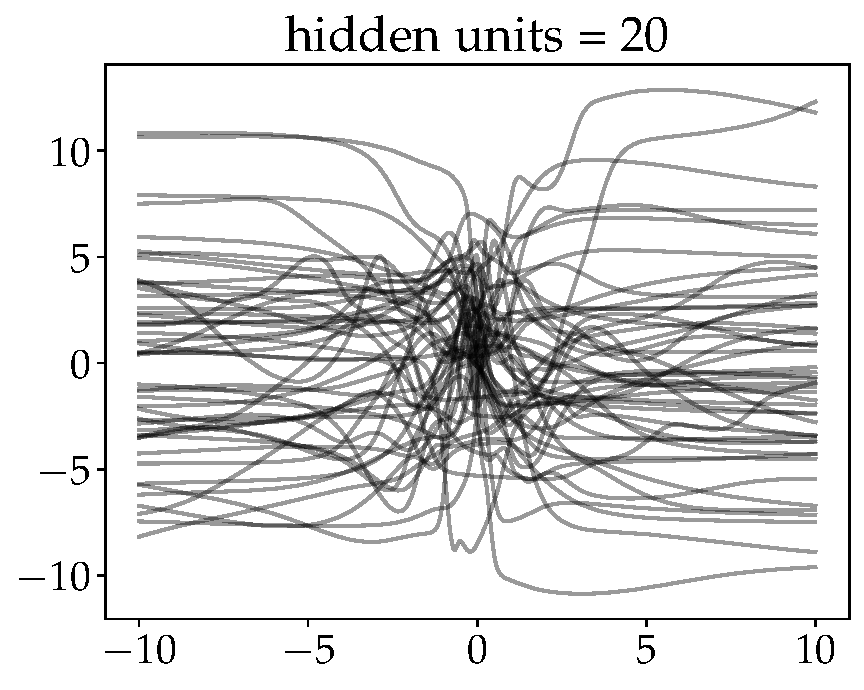
\includegraphics[width=\textwidth]{Pictures/bayesian_nn_prior_samples_hidden_units_2.pdf}
    \end{minipage}
    \hfill
    \begin{minipage}[b]{0.24\textwidth}
      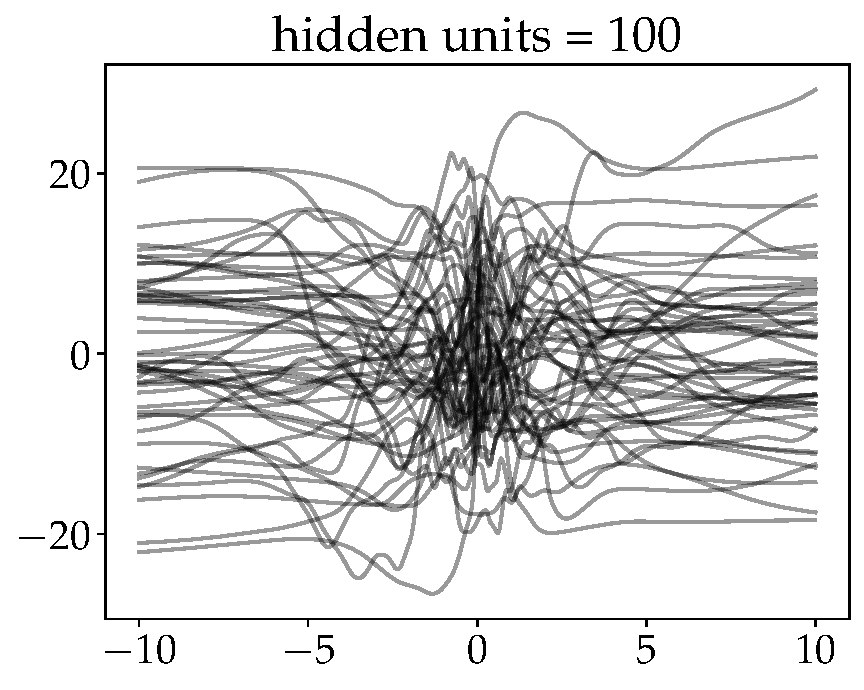
\includegraphics[width=\textwidth]{Pictures/bayesian_nn_prior_samples_hidden_units_3.pdf}
    \end{minipage}
    
    \caption{Prior samples from 3 layer BNN. The number of units in each of the three layers have a
    large influence on the BNNs ability to be expressive. Note that the inference becomes more
    computationally demanding with BNN size.}
    \label{n_unit_BNN}
  \end{figure}

% #\subsubsection{Expressiveness of BNN}
% The number of MCMC samples is of large importance. Theoretically speaking the more samples the better
% however, 

$\mathcal{N}(\textbf{w}|\bm{0},I)$, and the prior distribution of the observation
variance is following a inverse gamma distribution $\text{InvGa}(\sigma^2|1000,1)$ yielding a quite 
informative prior of $\sigma^2 \approx 0$, i.e. believing that there is no oberservation noise.

\begin{figure}[H]
    \centering
    \begin{minipage}[b]{0.49\textwidth}
     %\includegraphics[trim=1cm 0.7cm 1cm 1cm,clip,width=\textwidth]{Figures/reg_illustrations/BayesianNN_plots/Test4_BNN500-500-hu-10-alpha-1000_n_100_seed_42.pdf}
     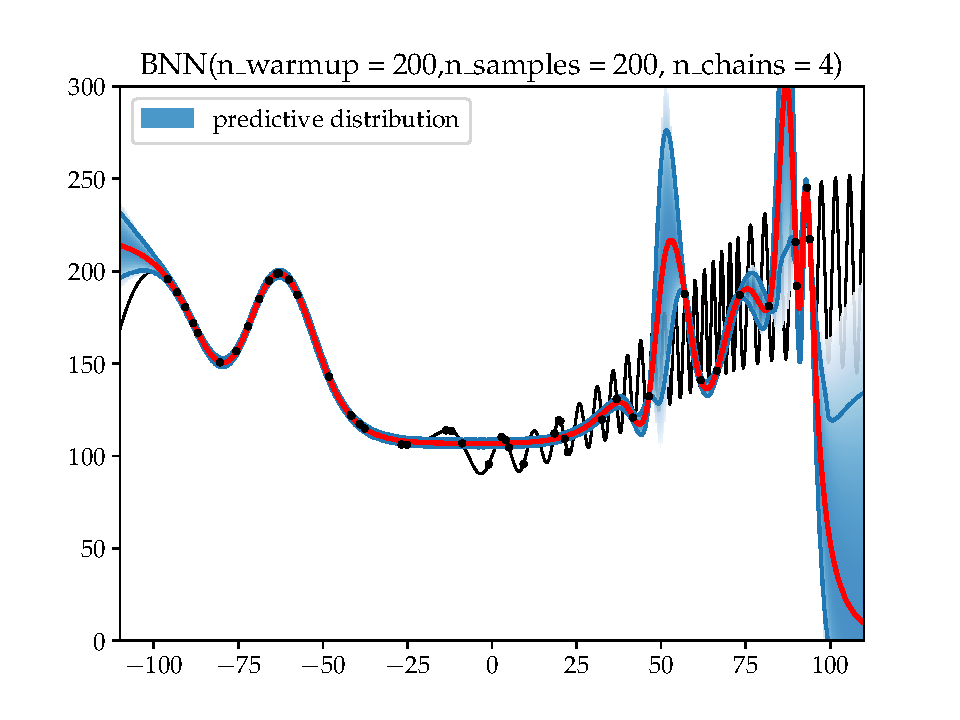
\includegraphics[width=\textwidth]{Pictures/Test4_BNNhu-10.pdf}
    \end{minipage}
    \hfill
    \begin{minipage}[b]{0.49\textwidth}
      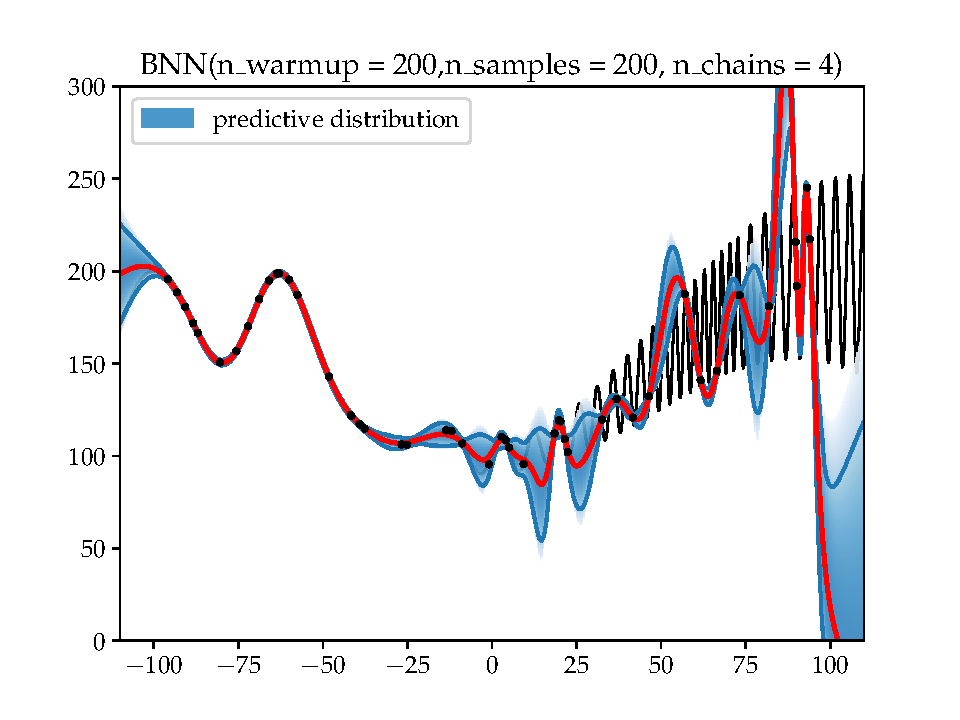
\includegraphics[width=\textwidth]{Pictures/Test4_BNNhu-50.pdf}
     \end{minipage}
     \caption{Example where 100 nodes on each of three layers, lead to a much more expressive model.
     $\sigma^2$ follows a informative prior $InvGamma(1000,1)$, i.e. prior mean $E[\sigma^2] \approx
     \frac{1}{1000}$, and variance $\approx \frac{1}{1000^3}$, however since the data is distributed in such 
     a complex way the limited expressiveness of the model, forces the model to infer make $\sigma^2$ large, 
     i.e. including the data in the noise}
\end{figure}

% Another variance! Sometimes the complexity of the problem is incapsled as noise.

% \subsubsection{Number of samples}
% The number of MCMC samples is of large importance. Theoretically speaking the more samples the better
% however, 


%\subsection{Benchmark BNN model}
